\section{Comparison of Available Wireless Communication Technologies}

There are three ways to communicate wirelessly underwater. These are
acoustic, optical and \ac{RF}.

\begin{figure}[H]
  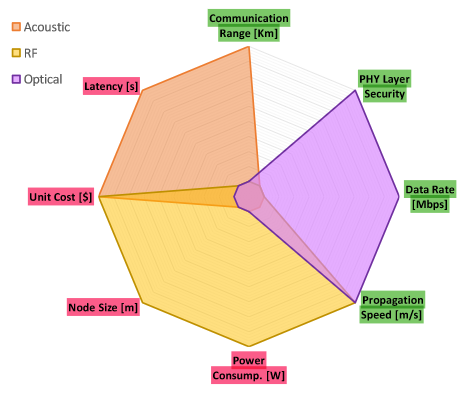
\includegraphics[width=0.8\textwidth]{acoustic_rf_optical_comparison.png}
  \caption{Comparison of Acoustic vs RF vs Optical Technologies}
  \label{fig:acoustic_rf_optical_comparison}
\end{figure}

\subsection{Above Surface to Underwater}

\subsection{Surface to Underwater}

\subsection{Hybrid Approaches}

\subsubsection{Control Plane versus Data Plane}
It is possible to utilise a hybrid approach to wireless underwater
communications. For example, we can use the much more reliable
acoustic link, which has a much lower data rate, for the control
plane. This gives reliability but a low throughput. The data plane
would then be over the optical link, giving high throughput with
much higher range than \ac{RF}.